\documentclass{uetgraduation}
\usepackage{graphicx}
\graphicspath{{graph/}}
\begin{document}
\studentname{Hoàng Trung Dũng}
\title{Nghiên cứu phương pháp chống nhiễu cho mạng truyền thông tán xạ ngược sử dụng phương pháp học sâu tăng cường}
\documenttype{Đồ án tốt nghiệp đại học hệ chính quy}
\major{Công nghệ thông tin}
\year{2024}
\supervisor{TS. Nguyễn Ngọc Tân}
\makecovers
% Tóm tắt
\begin{preamble}{Tóm tắt}
\textbf{Tóm tắt:} Truyền thông không dây đã và đang đóng vai trò vô cùng quan trọng trong cuộc sống con người. Tuy
nhiên phương pháp truyền thông này lại rất dễ bị tấn công gây nhiễu do tín hiệu vô tuyến phát sóng trong không gian mở.
Thêm vào đó, với sự phát triển của UAV (thiết bị bay không người lái) với khả năng cung cấp đường truyền tầm nhìn thẳng
(LoS) và hệ số suy giảm đường truyền thấp đã hỗ trợ cho việc tấn công đối với kết nối không dây. Trong khoá luận tốt nghiệp
này, em muốn trình bày một phương án chống nhiễu cho mạng truyền thông không dây, sử dụng học tăng cường sâu, kết hợp với
kỹ thuật tán xạ ngược và thu hoạch năng lượng để không những chống lại mà còn tận dụng được tín hiệu gây nhiễu từ UAV 
để nâng cao hiệu suất của hệ thống truyền thông không dây.

\textit{\textbf{Từ khóa:} Truyền thông không dây, Nhiễu, UAV, Học tăng cường sâu, Tán xạ ngược, Thu năng lượng.}
\end{preamble}
% Lời cảm ơn
\begin{preamble}{Lời cảm ơn}
    Đầu tiên, cho phép em gửi lời cảm ơn đến các thầy, cô giáo trường Đại học Công nghệ - Đại học
    Quốc Gia Hà Nội đã luôn tận tình chỉ bảo và tạo điều kiện trong suốt quá trình em học
    tập tại trường.
    
    Em xin gửi lời cảm ơn sâu sắc đến thầy giáo TS. Nguyễn Ngọc Tân đã tận tình
    hướng dẫn và đóng góp ý kiến quý báu trong suốt quá trình thực hiện khóa luận tốt
    nghiệp của em.
    
    Cuối cùng em xin gửi lời cảm ơn đến gia đình của mình, nơi đã luôn là nguồn động lực cho em
    trong suốt thời gian vừa qua.
    
    Em xin chân thành cảm ơn.
\end{preamble}
% Lời cam đoan
\begin{preamble}{Lời cam đoan}
Tôi xin cam đoan rằng mọi kết quả trình bày trong khóa luận đều do tôi thực hiện
dưới sự hướng dẫn của TS. Nguyễn Ngọc Tân.

Tất cả các tham khảo nghiên cứu liên quan đều nêu rõ nguồn gốc một cách rõ ràng từ 
danh mục tài liệu tham khảo trong khóa luận. Khóa luận không sao chép tài liệu, 
công trình nghiên cứu từ người khác mà không có rõ về mặt tài liệu tham khảo.

Các thông kê, các kết quả trình bày khóa luận đều là tự thực nghiệm khi chạy chương trình. Nếu tôi sai 
tôi hoàn toàn chịu trách nhiệm theo quy định của trường Đại học Công Nghệ - Đại học Quốc Gia Hà Nội.

\begin{flushright}
    Hà Nội, tháng 12 năm 2024

    \vspace{45pt}
    Hoàng Trung Dũng
\end{flushright}
\end{preamble}

% Muc luc
\begin{contentlisting}

\tableofcontents
\listoffigures
\listoftables

\begin{contentlistingsection}{Các từ viết tắt}
    UAV: unmanned aerial vehicle -- Thiết bị bay không người lái

    LoS: line-of-sight -- Đường truyền tầm nhìn thẳng

    MDP: Markov decision process

    RL: reinforcement learning -- Học tăng cường

    DRL: deep reinforcement learning -- Học tăng cường sâu.
    
    DQN: deep q network -- Mạng sâu Q.

    HTT: harvest then transmit -- Chiến lược thu năng lượng để truyền tin

    RA: rate adaption -- Kĩ thuật điều chỉnh tốc độ phát gói tin

    PSR: Packet Send Ratio -- Tỉ lệ gói tin được máy phát gửi

    PDR: Packet Delivery Ratio -- Tỉ lệ gói tin được gửi thành công đến máy thu

    MAC: medium access control -- Điều khiển truy nhập môi trường

    WLAN: wireless local area network -- Mạng cục bộ không dây

    WSN: wireless sensor network -- Mạng cảm biến không dây
\end{contentlistingsection}

\end{contentlisting}

% Chapter 1
\chapter{Đặt vấn đề}
Truyền thông không dây là thành phần không thể thiếu trong cơ sở hạ tầng viễn thông của xã hội ngày nay, có các ứng dụng và
tác động sâu rộng đến mọi mặt của đời sống con người. Mặc dù công nghệ truyền thông không dây đã có rất nhiều bước phát triển
qua nhiều thập kỉ, hầu hết các mạng truyền thông không dây vẫn dễ bị tấn công gây nhiễu bởi tính mở của nó. Bằng cách đưa tín
hiệu nhiễu vào kênh không dây đích, thiết bị gây nhiễu có thể làm giảm tỉ lệ tín hiệu trên nhiễu cộng nhiễu (SINR) của máy thu,
qua đó làm gián đoạn hoặc ngăn chặn kênh truyền không dây hợp lệ. Không giống như những tác động không có chủ đích, tín hiệu gây
nhiễu thường mạnh và qua đó có thể liên tục làm gián đoạn kênh truyền.

Gần đây, thiết bị bay không người lái (UAV) đang ngày càng được sử dụng nhiều hơn để nâng cao năng lực của hạ tầng mạng. Khả năng
triển khai nhanh cùng với tính cơ động cao của UAV khiến nó phù hợp với rất nhiều nhiệm vụ, ví dụ như việc triển khai hệ thống
mạng tạm thời ở những nơi khó tiếp cận như những vùng xảy ra thiên tai, bão lũ... UAV có thể cung cấp đường truyền LoS và hệ số suy
giảm kênh truyền thấp đến người dùng trên mặt đất khi nó được sử dụng như một trạm phát sóng. Do đó UAV có thể được sử dụng để
tăng cường năng lực của hệ thống mạng. Tuy nhiên chính những lợi thế của UAV như ở trên khiến cho nó có thể bị đối tượng xấu 
khai thác như là một thiết bị gây nhiễu di động, ngăn chặn đáng kể việc truyền dữ liệu và làm giảm chất lượng dịch vụ (QoS) của mạng
không dây, nghiêm trọng hơn so với gây nhiễu từ trên mặt đất. Vì thế giải quyết vấn đề gây nhiễu từ UAV là một bài toán đáng quan tâm.

Trong khoá luận này, em sẽ tìm hiểu về tấn công gây nhiễu, cũng như tấn công gây nhiễu từ UAV đối với mạng truyền thông không dây.
Qua đó đề xuất một phương án để không những chống lại mà còn tận dụng cuộc tấn công gây nhiễu để đảm bảo chất lượng đường truyền.
Phần còn lại của khoá luận sẽ được chia thành các chương với nội dung cụ thể như sau:

Chương 2: Cơ sở lý thuyết. Trong chương này trình bày lý thuyết nền tảng về tấn công gây nhiễu và tấn công gây nhiễu bằng UAV.
Cũng như tìm hiểu một số chiến lược chống nhiễu đã được nghiên cứu. Sau đó sẽ đi vào tìm hiểu về RL và DRL - hai phương pháp được
sử dụng để chống nhiễu.

Chương 3: Đề xuất phương án giải quyết bài toán tấn công gây nhiễu từ UAV. Trong chương này, em sẽ mô hình hoá bài toán tấn công
gây nhiễu bằng UAV và đề xuất phương pháp chống nhiễu sử dụng DRL.

Chương 4: Thiết lập mô phỏng và kết quả mô phỏng. Trong chương này, em sẽ trình bày chi tiết về mô hình và thông số thiết lập mô
phỏng phương pháp chống nhiễu được đề xuất. Cũng như so sánh hiệu quả mà phương pháp đề xuất mang lại so với chiến lược phòng thủ
''tham lam''.

Chương 5: Kết luận.

% Chapter 2
\chapter{Cơ sở lý thuyết.}
\section{Mạng không dây.}
\subsection{Giới thiệu.}
Mạng không dây là một hệ thống mạng truyền tải dữ liệu mà không sử dụng các dây cáp kết nối vật lý. Thay vào đó, mạng không dây sử dụng sóng
điện từ để truyền tín hiệu và dữ liệu giữa các thiết bị. Điều này giúp tăng tính di động của thiết bị, vốn là điểm yếu của các kết nối của các
kết nối có dây. Phương pháp gửi dữ liệu thông qua môi trường không khí này được ứng dụng vô cùng sâu rộng trong mọi lĩnh vực đời sống con người
ngày nay, từ công sở, trường học hoặc thậm chí là trong quân sự\dots

Dữ liệu nhận và gửi của mạng không dây được truyền đi xuyên suốt thông qua các tầng ảo sau:
\begin{itemize}
    \item Tầng vật lý: Là tầng thể hiện đặc điểm của kết nối vật lý giữa các thiết bị trong mạng, trong trường hợp mạng không dây, môi trường truyền
    là không khí. Quá trình nhận và truyền dữ liệu được quản lý bởi tầng vật lý. Trong mạng không dây, dữ liệu nhị phân giữa các thiết bị được chuyển
    thành tín hiệu điện và sử dụng tần số vô tuyến để gửi và nhận dữ liệu, tất cả quá trình này được thực hiện bởi tầng vật lý. Đây cũng là tầng chịu
    thiệt hại nặng nề nhất từ cuộc tấn công gây nhiễu sóng vô tuyến.
    \item Tầng liên kết dữ liệu: Là tầng ở giữa, chịu trách nhiệm kết nối giữa tầng vật lý và tầng mạng, ngoài ra còn thực hiện phân đoạn các gói được
    gửi bởi các tầng cao hơn thành các khung có thể được gửi bởi tầng vật lý. Tầng này cũng cung cấp khả năng kiểm tra lỗi và định dạng các khung dữ liệu
    được gửi. Tầng con MAC của tầng liên kết dữ liệu chịu trách nhiệm di chuyển các gói dữ liệu đến và đi từ nút này sang nút khác trên một kênh chung.
    Kênh truyền trong mạng không dây là một tần số mà các nút sử dụng để gửi dữ liệu. Tầng con MAC sử dụng giao thức MAC để đảm bảo tín hiệu gửi từ các
    trạm khác nhau trên cùng một kênh truyền không bị xung đột. Tầng này dễ bị tấn công gây nhiễu tầng liên kết dữ liệu - các thiết bị gây nhiễu tinh vi
    có thể tận dụng lợi thế của tầng liên kết dữ liệu và tạo ra cuộc tấn công hiệu quả về mặt năng lượng. So với tấn công gây nhiễu sóng vô tuyến ở tầng
    vật lý, gây nhiễu tầng liên kết dữ liệu tối ưu hơn về mặt năng lượng.
    \item Tầng mạng: Hoạt động như một liên kết giữa tầng giao vận ở trên và tầng liên kết dữ liệu ở dưới. Chịu trách nhiệm tìm ra cấu trúc mạng và gán địa
    chỉ, cũng như định tuyến dữ liệu.
    \item Tầng giao vận: Khôi phục dữ liệu bị mất và cũng chịu trách nhiệm truyền lại dữ liệu. Cung cấp khả năng mã hoá dữ liệu và truyền dữ liệu đáng tin cậy.
    \item Tầng ứng dụng: Tầng này chịu trách nhiệm xác định thông số kỹ thuật của dữ liệu được yêu cầu bởi cả người dùng cuối cũng như các nút trong mạng. 
\end{itemize}

\subsection{Phân loại mạng không dây và ứng dụng.}
\begin{itemize}
    \item WLAN: mạng không dây cục bộ, hay còn được biết đến nhiều hơn là Wi-Fi. WLAN cho phép thiết bị kết nối với Internet dễ dàng miễn là nó được kết nối với
    sóng Wi-Fi. WLAN được sử dụng ở rất nhiều nơi xung quanh chúng ta ngày nay, từ hộ gia đình, trường học, công sở, địa điểm kinh doanh\dots Thiết bị di động
    kết nối với điểm truy cập thông qua kết nối không dây sẽ có thể kết nối Internet và di chuyển một cách tự do, miễn là thiết bị đó ở trong tầm phủ sóng của
    sóng Wi-Fi.

    Hình 2.1 mô tả một mạng không dây cục bộ với một điểm truy cập và bốn thiết bị kết nối thông qua môi trường không dây.
    \begin{figure}{Mạng không dây cục bộ.}
        \centering
        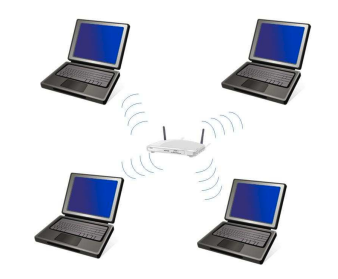
\includegraphics[scale=0.6]{wlan}
        \label{fig:wlan}
    \end{figure}
    \item WSN: Mạng cảm biến không dây, là một tập hợp số lượng lớn các nút có khả năng thu thập dữ liệu từ môi trường xung quanh và truyền tải thông tin
    về trung tâm xử lý dữ liệu hoặc các thiết bị thu thập dữ liệu. Trong WSN, các nút có thể chia sẻ thông tin cho nhau, dữ liệu thu thập từ các cảm biến không được
    gửi trực tiếp cho người dùng mà được xử lý và tổng hợp lại, chỉ gửi những thông tin mục tiêu mà mạng cảm biến muốn đạt được. Do đó những dữ liệu tạm thời, không
    cần thiết, chưa qua xử lý hoặc dữ liệu trung gian giữa các nút sẽ không được gửi tới người dùng.
    \begin{figure}{Mạng cảm biến không dây.}
        \centering
        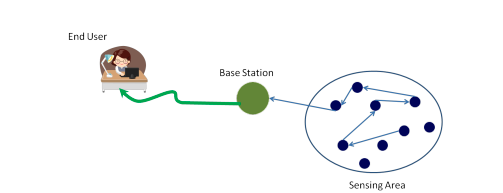
\includegraphics[scale=0.6]{wsn}
        \label{fig:wsn}
    \end{figure}

    Mạng cảm biến không dây có một số ứng dụng sau:
    \begin{itemize}
        \item Sử dụng trong lĩnh vực an ninh như giám sát ở các khu vực nhạy cảm để phát hiện các mối đe doạ như tấn công sinh học hoặc hoá học\dots
        \item Giám sát môi trường: WSN hỗ trợ thu thập thông tin ở những khu vực khó thiết lập cơ sở hạ tầng để giám sát môi trường cũng như môi trường sống.
        \item Trong y học: sử dụng để giúp các bác sĩ theo dõi sức khoẻ của bệnh nhân.
        \item Theo dõi đối tượng: WSN có thể dùng để theo dõi các đối tượng chuyển động nếu sử dụng cảm biến phù hợp.
        \item Hỗ trợ người khuyết tật: Người khuyết tật có thể độc lập hơn và cải thiện khả năng hoạt động với việc sử dụng WSN, WSN cho phép tự chăm sóc hiệu
        quả hơn và nâng cao chất lượng cuộc sống.
    \end{itemize}

    \item Mạng không dây tạm thời (ad hoc): là mạng không dây không cần bất kì cơ sở hạ tầng hiện có nào để triển khai ví dụ như điểm truy cập hoặc dây cáp.
    Mỗi thiết bị trong mạng coi là một nút tham gia trực tiếp vào việc định tuyến dữ liệu một cách độc lập bằng cách chuyển tiếp dữ liệu từ nút này sang nút khác
    mà không cần thêm bất kì một thiết bị quản lý tập trung nào như điểm truy cập\dots Mỗi nút trong mạng không dây tạm thời tự động quyết định nút nào sẽ gửi dữ
    liệu tiếp theo tuỳ thuộc vào kết nối mạng. Hình 2.3 là một mô hình đơn giản của mạng không dây tạm thời giữa các thiết bị kết nối với nhau mà không có điểm
    truy cập nào.
    \begin{figure}{Mạng không dây tạm thời.}
        \centering
        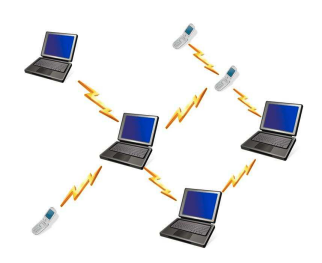
\includegraphics[scale=0.6]{ad_hoc}
        \label{fig:adhoc}
    \end{figure}

    Ứng dụng của mạng không dây tạm thời:
    \begin{itemize}
        \item Trong quân sự: người lính, các thiết bị quân sự như xe tăng, tàu chiến có thể kết nối với nhau mà không cần một cơ sở hạ tầng mạng không dây rõ ràng
        bằng cách hình thành một mạng không dây tạm thời.
        \item Mạng không dây tạm thời có thể được sử dụng trong các nhiệm vụ thực thi pháp luật, giải cứu\dots
        \item Có thể được sử dụng trong hội nghị, cuộc họp, bài giảng hoặc các khu vực phục vụ mục đích thương mại, nơi tải mạng có thể rất cao.
    \end{itemize}
\end{itemize}


\section{Tấn công gây nhiễu sóng vô tuyến.}
Trong mạng truyền thông không dây, đặc tính mở của môi trường truyền, cụ thể ở đây mạng không dây sử dụng không khí là môi trường truyền để truyền và nhận dữ
liệu, dẫn đến việc nó rất dễ bị tấn công bởi nhiều kiểu tấn công khác nhau. Ở đây chúng ta nghiên cứu cụ thể loại tấn công mạng không dây bằng gây nhiễu sóng
vô tuyến.

\subsection{Giới thiệu.}
Tấn công gây nhiễu sóng vô tuyến được định nghĩa là một hành động cố tình can thiệp vào quá trình truyền và nhận vật lý của truyền thông
không dây. Trong đó kẻ tấn công (máy gây nhiễu) sẽ phát tín hiệu vô tuyến trên cùng băng tần mà mạng mục tiêu sử dụng. Mục tiêu của việc
tấn công là làm giảm hiệu suất mạng hoặc thậm chí ngăn chặn hoàn toàn việc truyền thông tin không dây giữa các thiết bị.

Trong cuộc tấn công gây nhiễu, máy gây nhiễu đưa năng lượng gây nhiễu vào môi trường không dây, gây cản trở việc truyền tải hợp pháp theo
một trong hai cách: 
\begin{itemize}
    \item Máy gây nhiễu gửi tín hiệu nhiễu mạnh gây giảm tỉ lệ tín hiệu trên nhiễu cộng với nhiễu (SINR) ở máy thu.
    \item Gây nhiễu liên tục ngăn cản việc máy phát truy cập vào kênh truyền, dẫn đến một cuộc tấn công từ chối dịch vụ (DOS). Tấn công từ
    chối dịch vụ thực hiện bằng cách gửi tín hiệu nhiễu, gói tin giả khiến kênh truyền hợp lệ bận, làm cho máy phát ngừng gửi bất kì dữ liệu nào
    cho đến khi kênh truyền khả dụng trở lại.
\end{itemize}

Tấn công gây nhiễu sóng vô tuyến có một số đặc điểm sau đây:
\begin{itemize}
    \item Cố ý: Đây là hành động gây nhiễu có chủ đích của kẻ tấn công, nhằm vào một mục tiêu cụ thể, không giống với nhiễu tự nhiên gây
    ra bởi các yếu tố của môi trường.
    \item Không tuân thủ các giao thức MAC: đặc điểm chung của các cuộc tấn công gây nhiễu là việc liên lạc của chúng không tuân theo các
    giao thức MAC.
    \item Phạm vi tấn công: Máy gây nhiễu có thể nhắm vào một tần số cố định hoặc nhiều tần số khác nhau.
\end{itemize}

\subsection{Thông số đánh giá một cuộc tấn công gây nhiễu.}
Chúng ta xác định hai chỉ số để đánh giá hiệu quả của một cuộc tấn công gây nhiễu:
\begin{itemize}
    \item \textbf{SINR}: tỉ lệ tín hiệu trên nhiễu cộng nhiễu là tỉ số giữa công suất của tín hiệu máy phát so với tín hiệu gây nhiễu như
    tín hiệu từ máy gây nhiễu và nhiễu môi trường trong kênh truyền
    \[
    \theta = \frac{P_R}{\phi P_J + \rho^n},
    \]
    \item \textbf{PSR}: đại diện cho tỉ lệ giữa gói tin thực sự được gửi thành công bởi máy phát và số gói tin mà máy phát dự định gửi.
    Khi tín hiệu tấn công khiến cho kênh truyền giữa máy phát và máy thu bận
    \item \textbf{PDR}:
\end{itemize}


\subsection{Các mô hình tấn công gây nhiễu.}
Có rất nhiều chiến lược tấn công khác nhau mà máy gây nhiễu có thể thực hiện để làm nhiễu mạng không dây. Do đó cũng dẫn đến nhiều mô hình tấn công với
nhiều mức độ hiệu quả khác nhau. Tuy nhiên sau đây là một số mô hình gây nhiễu đã chứng minh được tính hiệu quả trong việc làm gián đoạn kết nối mạng không
dây.
\begin{itemize}
    \item \textbf{Máy gây nhiễu liên tục}: thiết bị gây nhiễu liên tục phát ra tín hiệu vô tuyến mà không có sự gián đoạn. Tín hiệu nhiễu phát ra có thể 
    là sóng điện từ đơn giản hoặc thậm chí là các bit dữ liệu. Sóng điện từ hoặc các bit dữ liệu được máy gây nhiễu phát ra này không tuân theo bất kì giao 
    thức hoặc quy tắc nào mà các nút trong mạng tuân theo. Kiểu máy gây nhiễu này làm giảm PDR bằng cách làm hỏng các bit tại máy thu, khiến máy thu không
    thể giải mã dữ liệu. Nó cũng có thể làm giảm PSR bằng cách giữ cho kênh truyền giữa máy phát và máy thu liên tục bận, ngăn chặn việc máy phát truyền sử
    dụng đường truyền hợp lệ để truyền gói tin đến máy thu.
    \item \textbf{Máy gây nhiễu lừa đảo}: loại máy gây nhiễu này rất giống với máy gây nhiễu liên tục do cùng liên tục truyền tín hiệu hoặc dữ liệu qua mạng.
    Tuy nhiên điểm khác biệt là máy gây nhiễu lừa đảo không truyền các bit dữ liệu ngẫu nhiên. Máy gây nhiễu giả mạo liên tục đưa các gói tin vào mạng mà không
    có bất kì khoảng cách nào giữa các lần truyền, và do dữ liệu không phải là các bit ngẫu nhiên, do đó khiến cho nút mạng tin rằng những bit dữ liệu này là
    hợp lệ và do đó không sử dụng đường truyền nữa. Ví dụ máy gây nhiễu có thể gửi gói tin ACK giả mạo để khiến máy phát tin rằng nó đã truyền dữ liệu thành công.
    \item \textbf{Máy gây nhiễu ngẫu nhiên}: hai kiểu máy gây nhiễu ở trên luôn luôn duy trì việc truyền tín hiệu hoặc dữ liệu vào mạng, dẫn đến việc nó không
    hiệu quả về mặt năng lượng và phải kết nối với nguồn năng lượng bên ngoài khiến nó hạn chế khả năng di chuyển. Máy gây nhiễu ngẫu nhiên mặt khác có chu kỳ ngủ
    và chu kỳ gây nhiễu, cả hai chu kỳ có thể tuân theo một phân phối xác suất hoặc có thể hoàn toàn là ngẫu nhiên. Việc có cả hai trạng thái ngủ và gây nhiễu
    khiến máy gây nhiễu có thể tắt tín hiệu gây nhiễu qua đó tiết kiệm năng lượng trong giai đoạn ngủ và hoạt động như bất kỳ máy gây nhiễu nào trong hai máy gây 
    nhiễu đã thảo luận ở trên trong chu kỳ gây nhiễu của nó.
    \item \textbf{Máy gây nhiễu phản ứng}: ba mô hình gây nhiễu ở trên là ba mô hình gây nhiễu chủ động theo nghĩa là chúng luôn chủ động tấn công kênh truyền
    bất kể lưu lượng qua kênh như thế nào. Gây nhiễu chủ động thường hiệu quả vì chúng khiến kênh truyền luôn bận rộn, tuy nhiên lại có nhược điểm là dễ bị phát
    hiện. Một cách tiếp cận khác so với gây nhiễu chủ động là gây nhiễu phản ứng, tức là không cần thiết phải tấn công kênh truyền khi không có lưu lượng trên đường
    truyền. Thay vào đó máy gây nhiễu phản ứng sẽ không hoạt động khi kênh truyền rảnh rỗi, và bắt đầu phát tín hiệu gây nhiễu ngay khi nó cảm nhận được hoạt động
    truyền phát tín hiệu trên kênh. Do đó nó nhắm vào việc nhận tin nhắn. Thiết bị gây nhiễu phản ứng có thể không tối ưu về mặt năng lượng do nó phải liên tục lắng
    nghe để cảm nhận kênh truyền. Tuy nhiên nó khó bị phát hiện hơn gây nhiễu chủ động.
\end{itemize}

\section{Tấn công gây nhiễu bằng UAV.}

\section{Kỹ thuật chống nhiễu.}

\subsection{Tán xạ môi trường xung quanh.}

\subsection{Thu hoạch năng lượng.}

\section{Markov decision process and Reinforcement learning.}

\section{Deep Reinforcement Learning}
\subsection{Deep Q Networking}

% Chapter 3
\chapter{Đề xuất phương pháp giải quyết bài toán gây nhiễu từ UAV.}
\section{Mô hình hệ thống.}
Ở đây, chúng ta xem xét một hệ thống truyền thông không dây bao gồm một máy phát, một máy thu và một UAV gây nhiễu. Máy phát được trang bị
bộ thu năng lượng và một mạch tán xạ ngược. Máy phát có thể thu năng lượng từ tín hiệu nhiễu và sử dụng năng lượng thu được này
để truyền gói tin chủ động đến máy thu - chế độ HTT, hoặc tán xạ ngược dữ liệu dựa trên sóng nhiễu - chế độ tán xạ ngược. Lưu ý
là máy phát chỉ có khả năng nhận biết cuộc tấn công có đang xảy ra hay không mà không biết được cụ thể cường độ tín hiệu nhiễu.

\subsection{Mô hình gây nhiễu.}

\subsection{Mô hình kênh truyền.}
Phần này trình bày chi tiết về kênh truyền giữa máy phát và máy thu, khi bị tấn công cũng như khi không bị tấn công


\section{Công thức hoá vấn đề.}
\subsection{Không gian trạng thái.}
Trình bày không gian trạng thái (state space) của bài toán

\subsection{Không gian hành động.}
Trình bày không gian hành động (Action Space)

\subsection{Phần thưởng tức thời.}


\subsection{Công thức tối ưu hoá.}


\section{Test}

% Chapter 4
\chapter{Thiết lập mô phỏng và đánh giá hiệu năng.}
\section{Thông số cài đặt thử nghiệm.}
Trong hệ thống đang được xem xét, máy phát có thể lưu trữ tối đa $D = 10$ gói tin trong hàng đợi dữ liệu, tối đa $E = 10$ đơn vị năng lượng
trong bộ lưu trữ năng lượng. Dữ liệu đến máy phát giả định tuân theo phân phối Poisson với tốc độ trung bình $\lambda = 3$ 
gói tin. Khi UAV gây nhiễu không tấn công, máy phát có thể truyền chủ động tối đa $\hat{d}_t = 4$ gói tin đến máy thu. Mỗi gói tin truyền đi cần
1 đơn vị năng lượng. Do sự thay đổi vị trí của UAV như đã nói ở trên, công suất gây nhiễu của UAV cũng thay đổi, giả định tín hiệu nhiễu từ 
UAV ảnh hưởng đến đường truyền không dây đang xét gồm bốn mức $P_J = \{0W, 5W, 10W, 15W\}$ với $P_{\text{max}} = 15W$. Do lượng năng lượng
thu hoạch được cũng như số gói tin tán xạ ngược thành công tăng lên khi tín hiệu nhiễu mạnh hơn, chúng ta đặt $e = \{0, 1, 2, 3\}$ là số đơn vị
năng lượng mà máy thu có thể thu được và $\hat{d} = \{0, 1, 2, 3\}$ là số gói tin mà máy thu có thể tán xạ ngược tương ứng với mức công suất nhiễu
ảnh hưởng tới đường truyền. Ngoài ra, khi UAV tấn công gây nhiễu và máy phát sử dụng kỹ thuật RA, nó có thể truyền $d^r_m = \{2, 1, 0\}$ gói tin
tương ứng với cường độ tín hiệu nhiễu từ UAV $P^J_n = \{5W, 10W, 15W\}$. Công suất nhiễu trung bình của UAV là $P_avg = 7.2W$.

\section{Kết quả mô phỏng.}
\subsection{Tốc độ hội tụ của hai phương pháp học tăng cường Q và DQN.}

\subsection{So sánh với chiến lược phòng thủ ''tham lam'' không sử dụng DRL.}
Ở đây, chúng ta thực hiện so sánh giữa việc sử dụng phương án DQN được đề xuất và chiến lược phòng thủ cố định ''tham lam'' được mô tả như sau: (i) Khi
UAV gây nhiễu không tấn công kênh truyền, máy phát sẽ phát chủ động gói tin đến máy thu, (ii) Khi UAV gây nhiễu tấn công kênh truyền, máy phát sẽ tận dụng
sóng nhiễu từ UAV để thu năng lượng hoặc tán xạ ngược đan xen nhau theo một chu kì cố định - máy phát sẽ tiến hành thu năng lượng từ sóng nhiễu sau mỗi chu kì
$T_\text{harvest} = 5$ đơn vị thời gian, thời gian còn lại máy phát sẽ tiến hành tán xạ ngược sóng nhiễu để truyền dữ liệu đến máy thu. Ta gọi chiến lược này
là chiến lược phòng thủ cố định ''tham lam''. Với phương án sử dụng DQN được đề xuất, em thực hiện $4 \times 10^4$ lần lặp để tìm ra chiến lược tối ưu cho máy
phát và sau đó so sánh hiệu quả với chiến lược tham lam đã nêu ở trên.

% Chapter 5
\chapter{Kết luận}

% Tài liệu tham khảo
\begin{thebibliography}{9}
\begin{bibsection}{Tiếng Anh}
    % Book
    \bibitem{hoang2023deep}
    Hoang, D.T. and Van Huynh, N. and Nguyen, D.N. and Hossain, E. and Niyato, D.
    \textit{Deep Reinforcement Learning for Wireless Communications and Networking: Theory, Applications and Implementation},
    \textit{Wiley}, 2023, pp. 37-163.
    % Paper
    \bibitem{Hossein22}
    Pirayesh, Hossein and Zeng, Huacheng
    ''Jamming Attacks and Anti-Jamming Strategies in Wireless Networks: A Comprehensive Survey'',
    \textit{IEEE Communications Surveys \& Tutorials},
    vol. 24, no. 2,
    pp. 767-809

    \bibitem{Vadlamani16}
    Satish Vadlamani,Burak Eksioglu,Hugh Medal,Apurba Nandi
    ''Jamming attacks on wireless networks: A taxonomic survey'',
    \textit{International Journal of Production Economics},
    vol. 172,
    2016,
    pp. 76-94

    \bibitem{Xu2005}
    Xu, Wenyuan and Trappe, Wade and Zhang, Yanyong and Wood, Timothy
    ''The feasibility of launching and detecting jamming attacks in wireless networks'',
    \textit{Association for Computing Machinery},
    2005,
    pp. 46–57
\end{bibsection}
\end{thebibliography}
\end{document}